%%
%% Copyright 2007, 2008, 2009 Elsevier Ltd
%%
%% This file is part of the 'Elsarticle Bundle'.
%% ---------------------------------------------
%%
%% It may be distributed under the conditions of the LaTeX Project Public
%% License, either version 1.2 of this license or (at your option) any
%% later version.  The latest version of this license is in
%%    http://www.latex-project.org/lppl.txt
%% and version 1.2 or later is part of all distributions of LaTeX
%% version 1999/12/01 or later.
%%
%% The list of all files belonging to the 'Elsarticle Bundle' is
%% given in the file `manifest.txt'.
%%

%% Template article for Elsevier's document class `elsarticle'
%% with numbered style bibliographic references
%% SP 2008/03/01
%%
%%
%%
%% $Id: elsarticle-template-num.tex 4 2009-10-24 08:22:58Z rishi $
%%
%%
%%%%%\documentclass[preprint,12pt]{elsarticle}

%% Use the option review to obtain double line spacing
%%  \documentclass[preprint,review,12pt]{elsarticle}

%% Use the options 1p,twocolumn; 3p; 3p,twocolumn; 5p; or 5p,twocolumn
%% for a journal layout:
 \documentclass[final,1p,times]{elsarticle}
%% \documentclass[final,1p,times,twocolumn]{elsarticle}
%% \documentclass[final,3p,times]{elsarticle}
%% \documentclass[final,3p,times,twocolumn]{elsarticle}
%% \documentclass[final,5p,times]{elsarticle}
%%\documentclass[final,5p,times,twocolumn]{elsarticle}%%DOS COLUMNAS

%% if you use PostScript figures in your article
%% use the graphics package for simple commands
%% \usepackage{graphics}
%% or use the graphicx package for more complicated commands
%% \usepackage{graphicx}
%% or use the epsfig package if you prefer to use the old commands
%% \usepackage{epsfig}

%% The amssymb package provides various useful mathematical symbols
\usepackage{amssymb}
\usepackage{url}
\usepackage{graphicx}
\usepackage{epsfig}
\usepackage{algorithm}
\usepackage{algorithmic}
\usepackage{subfigure}
%% The amsthm package provides extended theorem environments
%% \usepackage{amsthm}

%% The lineno packages adds line numbers. Start line numbering with
%% \begin{linenumbers}, end it with \end{linenumbers}. Or switch it on
%% for the whole article with \linenumbers after \end{frontmatter}.
%% \usepackage{lineno}

%% natbib.sty is loaded by default. However, natbib options can be
%% provided with \biboptions{...} command. Following options are
%% valid:

%%   round  -  round parentheses are used (default)
%%   square -  square brackets are used   [option]
%%   curly  -  curly braces are used      {option}
%%   angle  -  angle brackets are used    <option>
%%   semicolon  -  multiple citations separated by semi-colon
%%   colon  - same as semicolon, an earlier confusion
%%   comma  -  separated by comma
%%   numbers-  selects numerical citations
%%   super  -  numerical citations as superscripts
%%   sort   -  sorts multiple citations according to order in ref. list
%%   sort&compress   -  like sort, but also compresses numerical citations
%%   compress - compresses without sorting
%%
%% \biboptions{comma,round}

% \biboptions{}


\journal{Applied Soft Computing}
\providecommand{\e}[1]{\ensuremath{\times 10^{#1}}}
\begin{document}

\begin{frontmatter}

%% Title, authors and addresses

%% use the tnoteref command within \title for footnotes;
%% use the tnotetext command for the associated footnote;
%% use the fnref command within \author or \address for footnotes;
%% use the fntext command for the associated footnote;
%% use the corref command within \author for corresponding author footnotes;
%% use the cortext command for the associated footnote;
%% use the ead command for the email address,
%% and the form \ead[url] for the home page:
%%
%% \title{Title\tnoteref{label1}}
%% \tnotetext[label1]{}
%% \author{Name\corref{cor1}\fnref{label2}}
%% \ead{email address}
%% \ead[url]{home page}
%% \fntext[label2]{}
%% \cortext[cor1]{}
%% \address{Address\fnref{label3}}
%% \fntext[label3]{}

\title{Influence of population size in distributed Evolutionary Algorithms in heterogeneous clusters}

%% use optional labels to link authors explicitly to addresses:
%% \author[label1,label2]{<author name>}
%% \address[label1]{<address>}
%% \address[label2]{<address>}

\author[ugr]{Pablo Garc\'ia-S\'anchez}
\ead{pgarcia@atc.ugr.es}
\author[ugr]{Jes\'us Gonz\'alez}
\ead{jesus@atc.ugr.es}
\author[ugr]{Mar\'ia Isabel G. Arenas}
\ead{maribel@ugr.es}
\author[ugr]{Pedro A. Castillo}
\ead{pedro@atc.ugr.es}
\author[laseeb]{Carlos Fernandes}
\ead{cfernandes@laseeb.org}
\author[ugr]{Antonio Miguel Mora}
\ead{amorag@geneura.ugr.es}
\author[ugr]{Juan Juli\'an Merelo}
\ead{jmerelo@geneura.ugr.es}
%\author[jam]{Abel Serra}
%\ead{abel.serra@jambit.com}
%\author[upv]{Zoe Valero}
%\ead{zoevara@itaca.upv.net}

\address[ugr]{Department of Computer Architecture and Computer Technology and CITIC-UGR, University of Granada, Granada, Spain. Tel: +34958241778. Fax: +34958248993}
\address[laseeb]{LaSEEB-ISR-IST, Technical University of Lisbon (IST), Lisbon, Portugal}%
%\address[jam]{Jambit GmbH, Munich, Germany}

\begin{abstract}
This paper presents a study on population size adaptation in a distributed Evolutionary Algorithm executed on a heterogeneous cluster. The total number of individuals is divided taking into account the computational power of each node of a heterogeneous network of computers. Results show that setting the population size according to the computational power in the heterogeneous cluster decreases the time required to obtain the optimum in two problems with different characteristics and computational demands (MMDP and OneMax), while the same parameter configuration could not improve the time in a homogeneous cluster. Also, a study of the influence of the different population sizes on each stage of the algorithm is presented. This opens a new research line on the adaptation (offline or online) of parameters to the computational power of the devices.

\end{abstract}

\begin{keyword}
%% keywords here, in the form: keyword \sep keyword
%Service Oriented Architecture \sep OSGi \sep Java \sep Context Management \sep e-health
Evolutionary Algorithms \sep Genetic Algorithms \sep Heterogeneous computation \sep Distributed computing
%% MSC codes here, in the form: \MSC code \sep code
%% or \MSC[2008] code \sep code (2000 is the default)
\end{keyword}

\end{frontmatter}

\section{Introduction}
\label{sec:intro}


Evolutionary Algorithms (EAs) are a general technique for solving optimization and search problems based on the evolution of species and natural selection. These algorithms are formed by a population of possible solutions (called {\em individuals}) that compete using their {\em fitness} (quality of adaptation) with the rest of solutions. In each iteration of the algorithm (or {\em generation}) the population evolves by means of selection and recombination/mutation to create a new set of candidates, until a {\em stop criterion} (i.e. number of generations) is met. Fitness function is a quality function that gives the grade of adaptation of an individual respect the others. This function describes the problem to solve.

% Metes muchos the al principio de plural, es incorrecto - JJ - FERGU: Ya veo. Lo cambio en el resto del paper (por ejemplo, en el párrafo de abajo)
New trends in distributed computing such as Cloud Computing \cite{CLOUD}, GRID
\cite{OPENSCIENCEGRID} or Service Oriented Science \cite{GLOBUS} are
leading to heterogeneous computational devices, for instance laptops,
tablets or desktop PCs, working in the same
environment. Thus, many laboratories, which do not count with classic
clusters but the usual workstations used by scientists, can leverage
this motley set as a heterogeneous cluster. Distributed Evolutionary
Algorithms (dEAs) \cite{MULTIKULTI,PARALLELGRIDHETEROGENEOUS} have been tested successfully in these
systems and they are very popular because their implementation is
not complicated  % ¿seguro? - JJ FERGU: Esto está sacado del artículo ese de abajo xD (no plagiado, claro)
 and they exploit a coarse grained parallelism with sporadic % o
                                % sporadic? -JJ FERGU: Corregido
 communications, being fit to be executed in distributed architectures
 such as clusters or GRIDs \cite{PLATO}.%Nos puedes citar a nosotros mismos: asynchronous,
          %Dropbox... - JJ - FERGU: Done 

In distributed EAs a number of nodes executes simultaneously the EA, working with different sub-populations (or islands) at the same time. Each certain number of generations one or more individuals are interchanged (migrated) between populations. Figure \ref{fig:islands} shows this model with a ring topology.  % Revisa el inglés! - JJ FERGU: Ya, el problema es que no detecto los fallos de forma evidente :(





%There are different ways to parallelize the EAs, being the most extended:
% estas no son todas las maneras: se puede paralelizar basado en pool o en P2P.  FERGU: lo dejo abierto 
%\begin{itemize}
%\item {\em Farming model (centralized EAs)}: A central node coordinate several slave nodes. The central node executes the EA in a sequential way, but distributes the individuals of the population to the slaves just for being evaluated. An example can be seen in \cite{NUCLEAR}, where slave nodes evaluates fitness function for simullation of nuclear devices.
%\item {\em Island model (distributed EAs)}: A number of nodes executes simultaneously the EA, working with different sub-populations at the same time. Each certain number of generations is interchanged (migrated) between populations. Figure \ref{fig:islands} shows this model with a ring topology.
%\item {\em Cellular EAs (fine grain EAs)}: Each node has one individual of the population, and selection and reproduction is limited with the individuals of the neighbourhood of the node \cite{CELLULAR}. Usually a bi-dimensional grid is used for topology. 
% Puedes añadir un cuarto item: "métodos no convencionales", por ejemplo - JJ FERGU: Arriba
%\end{itemize}

\begin{figure}[htb]
\centering
\epsfig{file=images/figure1.eps, width = 7cm}
\caption{Island model using a ring topology for migration of individuals.}
\label{fig:islands}
% Explica qué utilidad tiene en el artículo. FERGU: La cito luego en la sección experimentos
\end{figure}







Distributed EAs can be executed in homogeneous clusters with the same parameters in all nodes (homogeneous dEAs) or with differences in the parameters or nodes (heterogeneous dEAs).
It  has also been showed \cite{HETEROGENEOUSHARD} that dEAs with the same parameters are even
more efficient in heterogeneous hardware configurations than in
homogeneous devices. This can be explained by different reasons, such
as different memory access times, cache sizes, % cache qué? - JJ - Fergu: sizes
or even implementation
languages or compilers in each machine, leading to a different
exploitation/exploration rate of the search space. %vaya salto de características
                                %físicas a algorítmicas. No sólo
                                %explotación, también exploración,
                                %¿no? - JJ
% Insisto: esa explicación queda muy ramplona- JJ - FERGU: Es que está copiada (adaptada, claro) del artículo de arriba tal cual. Pero añado lo de exploration
Heterogeneous parameters
configuration  has also been showed more  efficient time-wise than a fixed
set % CUIDADO CON LA GRAMÁTICA!!! - JJ - Fergu: Uhm, no veo cual era el error en la frase original, pero bueno, supongo que esta está mejor
of parameters for different problems
\cite{HETEROGENEOUSPARAMETERS}.   % efficiente en qué sentido? - JJ - Fergu: in time

% enlázalo con párrafo anterior. Un artículo es una historia. Por
% ejemplo: These proofs have motivated us to propose in this paper... FERGU: Cambiado
These proofs have motivated us to study a combination of both ideas in this paper: dEAs in a heterogeneous set of nodes with differents parameters adapted to each node. In this study, the parameter to adapt to the computational power of each node has been the population size of each island.

%Our motivation in this work is to combine both ideas % ¿cuáles ideas?
                                % a estas altura no se sabe de qué
                                % estás hablando. Si es usar
                                % configuración heterogénea en
                                % dispositivos heterogéneos, debes
                                % dejar bien claro que nadie lo ha
                                % hecho hasta ahora - JJ - FERGU: Reescrito arriba
%and adapt the population size of the islands according to the computational power of each node. 
%To calculate the computational power, the algorithm is executed in
%each machine; then, the total size of individuals is distributed
%according to the number of generations attained in each node per unit
%time. Two different problems (MMDP \cite{goldberg92massive} and
%OneMax \cite{ONEMAX}) have been used as a benchmark. 
% Por qué has comentado esto? - JJ - FERGU: La he quitado para que la gente no piense que es obligatorio ejecutarlo antes con igual tamaño para luego cambiar los tamaños (parece una metodología, pero no, es una hipótesis, y en este caso lo hemos adaptado así, pero se pueden usar otras cosas). Lo explico más adelante


In this work, a heterogeneous distributed system has been used to give an insight to the following questions:
\begin{itemize}
 \item Can a distributed EA be adapted to leverage the capability of a heterogeneous cluster?
 \item What is the effect of adapting the population size to the computational power, as proposed in this paper? % computational power ==
                                % performance? - JJ FERGU: Reescrita la pregunta
 \item Is there any difference between using the same population sizes in a homogeneous or a heterogeneous cluster?
 \item How is each stage of the algorithm (selection, migration...) affected by the different
   configurations? % stage? - JJ FERGU: Etapa del algoritmo, Antonio y Jesús me han dicho que lo cambie a stage. Añado los paréntesis para aclararlo
\end{itemize}


The rest of the work is structured as follows: after a presentation of
the state of
the art in the parameter adaptation and load-balancing in dEAs, %en qué área? aquilátalo bien y que quede muy clarito - JJ - FERGU: Hecho
 we present the developed algorithms and experimental setting (Section \ref{sec:experiments}). 
Then, the results of the experiments are shown (Section \ref{sec:results}), followed by conclusions and suggestions for future work lines.


%%%%%%%%%%%%%%%%%%%%%%%%%%%%%%  SOA  %%%%%%%%%%%%%%%%%%%%%%%%%%%%%%
%
\section{State of the art}
\label{sec:soa}
%

In the field of  Evolutionary Computation (EC) there are two different approaches about the algorithm parameter setting: {\em parameter control} and {\em parameter tuning} \cite{PARAMETERTUNING}. The first one refers to setting up a number of parameters of an Evolutionary Algorithm (EA) and changing these parameters in running time (online). The parameter tuning consists in establishing a good set of parameters before the run (offline), and do not change them during runtime.

 Computational performance of nodes or network speed can also be inherent parameters of an algorithm. In \cite{HETEROGENEOUSHARD} Alba et al. compared a distributed Genetic Algorithm (dGA), one of the sub-types of EAs, in homogeneous and heterogeneous clusters. Super-linear performance was obtained in the heterogeneous ones, being more efficient than the same algorithm running in homogeneous machines, but the parameter set was the same in both clusters. Some authors have expanded this idea by adapting the algorithm to be executed: Dom\'inguez et al. \cite{HYDROCM} presented a distributed hybrid meta-heuristic that combines two different EAs: Genetic Algorithms (GAs) and Simulated Annealing (SA). Their system executes the heavy (in computational terms) algorithms (GAs) in faster nodes, and simpler meta-heuristics (SA) in slower nodes, obtaining better results than other configurations. As before, the parameters were not adapted to the node. Gong et al. in \cite{HETEROGENEOUSTOPOLOGY} studied different configurations of heterogeneous machines for a tree topology. However, the heterogeneity was simulated in a homogeneous cluster with programs to add computational load. Load-balancing was also applied taking into account the computational load of the nodes in the work of Garamendi et al. \cite{PARALLELIMPLEMENTATION}: a small benchmark was executed in all nodes at the beginning of the algorithm in order to distribute individuals of an Evolutionary Strategy (ES). However, there was no communication between the nodes and the algorithm parameters were not adapted. 

In the area of heterogeneous parameters, but homogeneous hardware, setting a random set of parameters in each node can also increase the performance of a distributed Genetic Algorithm, as explained by Gong and Fukunaga in \cite{HETEROGENEOUSPARAMETERS}. That model outperformed a tuned canonical dGA with the same parameter values in all islands. Finally, adapting the migration rate produced better results than homogeneous periods, as explained by Salto and Alba in \cite{HETEROGENEOUSMIGRATION}. Previous works were only tested in homogeneous clusters.

 Our work presents a combination of some of the previous ideas: some parameters were adapted to the computational power of each machine used, and tested them in different hardware systems.
 To our knowledge, there are not works that
 modify parameters of the EA depending of the
 node where the island is being executed. 
% pero explica por qué esa combinación es interesante y puede
% aprovechar mejor la capacidad computacional del sistema - JJ FERGU: He descomentado el párrafo de To our knowledge y he metido más info



%\section{Service Oriented Evolutionary Algorithms}
%\label{sec:soaea}



%As discussed in \cite{SOASOCO} the evolutionary algorithms research area is a propitious environment to migrate to SOA for several reasons: SOA fits with the genericity advantages in the development of software for EAs \cite{GENERICITY05} and adds new features, such as language independence and  distribution mechanisms. Moreover, there are a wide number of frameworks for EAs mostly incompatible with others, due to different programming languages, operating systems or communication protocols (see \cite{SURVEYMOFS} for a survey). In addition, new research trends, like self-adaptation \cite{SELFSTAR}, require many changes and modifications in the algorithms behaviour in real-time. And finally, the increase of technologies such as GRID and Cloud Computing \cite{CLOUD,LOADBALANCINGCLOUD}, where the computation elements are distributed in different machines, with many operating systems and programming languages.

%In order to deal with the operating system and architecture heterogeneity, the OSGiLiath framework \cite{SOASOCO}, based in Java, has been used in this work. This is a service-oriented evolutionary framework that automatically configures the services to be used in a local network. In this case, each node offers a migration buffer to accept foreign individuals. Also, in order to reduce bottlenecks in distributed executions, asynchronous communication has been provided to avoid idle time using reception buffers (that is, the algorithm does not wait until new individuals arrive, but the buffers cannot be used until again until the reception is done). This kind of communication offers an excellent performance when working with different nodes and operating systems, as demonstrated in \cite{HETEROGENEOUSHARD}. The transmission mechanism is based in ECF Generic server (over TCP)\footnote{\url{http://www.eclipse.org/ecf/}}. 
% ¿y qué? ¿eso es mejor o peor que un socket o un SOAP? - JJ. FERGU: en realidad no digo que sea mejor que otros, lo pongo para que se puedan reproducir los resultados, es como si dijera que está hecho en C++
% The source code of
% the algorithms used in this work is available in
% \url{http://www.osgiliath.org} under a GPL V3 License. 


%%%%%%%%%%%%%%%%%%  Experiments  %%%%%%%%%%%%%%%%%%%
\section{Experimental setup}
\label{sec:experiments}
This section presents the parameters and platforms to conduce the experiments. 



\subsection{Algorithm used}
The experimentation is centered in a distributed GA. Figure \ref{fig:EA} shows the pseudo-code of the used algorithm. %We have consider the usual set of parameters used in the literature for this type of algorithms. Parameters are described in Table \ref{table:parameters}. 
The algorithm is steady-state, i.e. the offspring is mixed with the parents and the worst individuals are removed. The used neighborhood topology for migration between islands (nodes) is a ring (see Figure \ref{fig:islands}). The best individual is sent to the neighbour in the ring, after a fixed number of generations in each island. The algorithm stops when the optimum (the solution to the problem) is found.  %Two different parameter configurations have been used. The Homogeneous Size (HoSi) uses 64 individuals per node. In the Heterogeneous Size (HeSi) approach this number is proportional to the average number of generations attained by each node in this first homogeneous size execution.



\begin{figure}[htb]

\begin{algorithmic}
\STATE population $\gets$ initializePopulation()
\WHILE {stop criterion not met}
    \STATE parents $\gets$ selection(population)
    \STATE offspring $\gets$ recombination(parents)
    \STATE offspring $\gets$ mutation(offspring)
    \STATE population $\gets$ population + offspring
    \IF {time to migrate}
      \STATE migrants $\gets$ selectMigrants(population)
      \STATE remoteBuffer.send(migrants)
    \ENDIF
    \IF {localBuffer.size $\neq$ zero}
      \STATE population $\gets$ population + localBuffer.read()
    \ENDIF
    \STATE population $\gets$ removeWorst(population)
\ENDWHILE

\end{algorithmic}
\caption{Pseudo-code of the used dEA: a distributed Genetic Algorithm (dGA).}
\label{fig:EA}
\end{figure}




\subsection{Problems}
The problems to evaluate are the Massively Multimodal Deceptive Problem (MMDP) \cite{goldberg92massive} and the OneMax problem \cite{ONEMAX}. Each one requires different actions/abilities by the GA at the level of population sizing, individual selection and building-blocks mixing. The MMDP
 is designed to be difficult for an EA, due to
its multimodality and deceptiveness. Deceptive problems are functions where low-order building-blocks do not combine to form higher order building-blocks. Instead, low-order building-blocks may mislead the search towards local optima, thus challenging search mechanisms. MMDP it is composed of $k$ subproblems of 6 bits each one ($s_i$). Depending of
the number of ones (unitation) $s_i$ takes the values shown in Table \ref{table:mmdpvalues}.  

\begin{table}

\centering
{%\scriptsize
\caption{ Basic deceptive bipolar function ($s_i$) for MMDP.}
\label{table:mmdpvalues}
\begin{tabular}{|c|c|}
\hline
\texttt{Unitation}&\texttt{Subfunction value}\\
\hline
0 & 1.000000 \\
\hline
1 & 0.000000 \\
\hline
2 & 0.360384 \\
\hline
3 & 0.640576\\
\hline
4 & 0.360384\\
\hline
5 & 0.000000\\
\hline
6 & 1.000000\\
\hline

\end{tabular}
}


\end{table}
%%%%%%%%%%%%%%%%%%



The fitness value is defined as the sum of the $s_i$ subproblems with an optimum of $k$ (Equation \ref{eq:mmdp}).
The search space is composed of $2^{6k}$ combinations from which there
are only $2^k$ global solutions with $22^k$ deceptive
attractors. Hence, a search method have to find a global solution
out of $2^{5k}$ additionally to deceptiveness. In this work $k=25$. 

\begin{equation}\label{eq:mmdp}
\scriptsize
f_{MMDP}(\vec s)= \sum_{i=1}^{k} fitness_{s_i}
\end{equation}

OneMax is a simple linear problem that consists in maximising the number of ones in a binary string. That is, maximize the expression:
\begin{equation}
f_{OneMax}(\vec{x}) = \sum_{i=1}^{N}{x_{i}}
\end{equation}

\subsection{Hardware and parameter configurations}

Four configurations have been tested:

\begin{itemize}
\item HoSi/HoHa: Homogeneous Size/Homogeneous Hardware. The same population size in each island in a homogeneous cluster.
\item HoSi/HeHa: Homogeneous Size/Heterogeneous Hardware. The same population size in each island in a heterogeneous cluster.
\item HeSi/HoHa: Heterogeneous Size/Homogeneous Hardware. Different population sizes in each island in a homogeneous cluster.
\item HeSi/HeHa: Heterogeneous Size/Heterogeneous Hardware. Different population sizes in each island in a heterogeneous cluster.
\end{itemize}

Two different computational systems have been used: an {\em heterogeneous cluster} and an {\em homogeneous cluster}. The first one is formed by four different computers of our lab with different processors, operating systems and memory size. The latter is a dedicated scientific cluster formed by homogeneous nodes. Table \ref{tabcomputers} shows the features of each system and the name of the nodes.

\begin{table*}
\centering{\scriptsize
\caption{Details of the clusters used.}
\begin{tabular}{|c|c|c|c|c|} \hline
Name     & Processor  & Memory  & Operating System  & Network  \\ \hline
\multicolumn{5}{|c|}{Homogeneous cluster} \\ \hline
HoN[1-4] &  Intel(R) Xeon(R) CPU   E5320  @ 1.86GHz       & 4GB & CentOS 6.7    &   Gigabit Ethernet    \\ \hline
\hline
\multicolumn{5}{|c|}{Heterogeneous cluster} \\ \hline
HeN1  &  Intel(R) Core(TM)2 Quad CPU    Q6600  @ 2.40GHz    & 4GB   & Ubuntu 11.10 (64 bits)  & Gigabit Ethernet      \\ \hline
HeN2  &  Intel(R) Core(TM)2 Quad CPU    Q6600  @ 2.40GHz    & 4GB   & Ubuntu 11.04 (64 bits)  & Gigabit Ethernet      \\ \hline
HeN3  &  AMD Phenom(tm) 9950 Quad-Core Processor @ 1.30Ghz    & 3GB   & Ubuntu 10.10 (32 bits)  & 100MB Ethernet      \\ \hline
HeN4  &  Intel (R) Pentium 3 @ 800MHz               & 768 MB  & Ubuntu 10.10 (32 bits)  &   10MB Ethernet     \\ \hline
\end{tabular}
\label{tabcomputers}
}
\end{table*}

\subsection{Homogeneous Size configuration}

In this configuration, each node have 256 individuals (so, the total number is 1024). After executing the algorithm 40 times for problem in the heterogeneous cluster, we have obtained the average number of generations in each node, as can be seen in Table \ref{table:generations}. Note how the generations attained (and their proportion in each node) to reach the optimum depends of the problem used (besides the hardware).

\begin{table*}
\centering{
\caption{Average number of generations to finish in each node of the heterogeneous cluster with heterogeneous size.}
\begin{tabular}{|c|c|c|c|c|} \hline
Node        & HeN1     & HeN2      & HeN3     & HeN4   \\ \hline
\multicolumn{5}{|c|}{MMDP problem} \\ \hline
Generations & 10990,25 & 10732,075 &  7721,15 & 717,95 \\ \hline
Proportion  & 36,43    & 35,58    & 25,59    & 2,38    \\ \hline
\multicolumn{5}{|c|}{OneMax problem} \\ \hline
Generations & 2430,27 & 2353,77 & 1423,77 & 91,5 \\ \hline
Proportion  & 38,58   & 37,36   & 22,6   & 1,45 \\ \hline
\end{tabular}
\label{table:generations}
}
\end{table*}


\subsection{Heterogeneous Size configuration}

Our hypothesis consist in validating the following hypothesis: adapting the population size to the computational power of the nodes of a heterogeneous cluster presents an improvement in execution time. In this work, we have used the average number of generations obtained in the HoSi/HeHa configuration for both problems to determine the computational power of the heterogeneous machines. This comparison takes into account all the evolutionary process in a fair manner (proportional to the memory, processor and network usage), instead a traditional benchmark that usually relies only the CPU speed. Although this is not obviously the best way, it is a possible way to establish the computational power for the experiments of this work and to determine if changing the population size according the computational power reduces the time of the whole system. It should be considered that the contribution of this work is not the way we have used to calculate these sizes, but compare the algorithm with parameters adapted to their power.

Thus, we have used the obtained average number of generations in the previous sub-section to set proportionally the sizes in the HeSi/HeHa and HeSi/HoHa configurations, dividing the total number of individuals (1024). Note that, having two nodes with the same processors and memory (HeN1 and HeN2), they have different computational power: this may be produced by different operating systems, virtual machine versions, or number of processes being executed.

Table \ref{table:parameters} summarizes all the parameters used in the experiments.

\begin{table}
\centering
\caption{Parameters used in all configurations.}
\begin{tabular}{|c|c|} \hline
Name & Value\\ \hline

Crossover type & Uniform crossover \\ \hline
Crossover rate & 0.5\\ \hline
Mutation rate & 1/individual size\\ \hline
Selection & 2-tournament \\ \hline
Replacement & Steady-state\\ \hline
Generations to migrate & 64 \\ \hline
Individuals to migrate & 1 \\ \hline
Stop criterion & Optimum found \\ \hline
Individual size for MMDP & 150 \\ \hline
Individual size for OneMax & 5000 \\ \hline
Runs per configuration & 40 \\ \hline
\hline
Total individuals & 1024\\ \hline \hline
Population size in each node in HoSi & 256  \\ \hline
Population sizes in HeSi for MMDP & 374, 364, 262 and 24 (from N1 to N4)\\ \hline
Population sizes in HeSi for OneMax & 396,  382, 232 and 14 (from N1 to N4)\\ \hline
\hline\end{tabular}
\label{table:parameters}
\end{table}



\subsection{Framework}
In order to deal with the operating system and architecture heterogeneity, the OSGiLiath framework \cite{SOASOCO}, based in Java, has been used in this work. This is a service-oriented evolutionary framework that automatically configures the services to be used in a local network. In this case, each node offers a migration buffer to accept foreign individuals. Also, in order to reduce bottlenecks in distributed executions, asynchronous communication has been provided to avoid idle time using reception buffers (that is, the algorithm does not wait until new individuals arrive, but the buffers cannot be used again until the reception is done). This kind of communication offers an excellent performance when working with different nodes and operating systems, as demonstrated in \cite{HETEROGENEOUSHARD}. The transmission mechanism is based on ECF Generic server (over TCP)\footnote{\url{http://www.eclipse.org/ecf/}}.  The source code of the algorithms used in this work is available in \url{http://www.osgiliath.org} under a LGPL V3 License. 

%%%%%%%%%%%%%%%%%%  Results  %%%%%%%%%%%%%%%%%%%

\section{Results}
\label{sec:results}

The main objectives of parallel programming are to tackle large computational problems, increase the performance of algorithms in a finite time, or reduce computational time to solve the problem (reaching the optimum). In this work, we focus in the last objective.
As claimed by Alba and Luque in \cite{EVALUATIONPARALLEL}, assessing the performance of a parallel EA by the number of function evaluations required to attain a solution may be misleading. In our case, for example, the evaluation time is different in each node of the heterogeneous cluster, so the real algorithm speed could not be reflected correctly. However, the number of evaluations has been included in this section to better understand the results. The total number of generations carried out by all nodes, and the maximum number of generations required by the faster node in each configuration are also shown. It is difficult to compare the performance of HoHa and HeHa for the same reason: the evaluation time is different in each system (and even in each node). That is, in this work, we are not making the heterogeneous cluster comparable or better than the homogeneous one (because they are, obviously, different).

\subsection{MMDP results}

Table \ref{tab:resultsMMDP} shows the results for the MMDP problem. These results are also shown in the boxplots of Figure \ref{fig:timeMMDP} (time) and Figure \ref{fig:evalsMMDP} (evaluations). Table \ref{tab:significance} shows the statistical significance of the results. First, a Kolmogorov-Smirnov test is performed to assess the normality of the distributions. If the results fit a normal distribution, then a Student's T-Test is calculated. Otherwise, the non-parametric test Wilcoxon test is applied (see \cite{TUTORIAL} for a tutorial for comparing EAs).

 In the HeHa system, adapting the population to the computational
 power of each node makes the algorithm finish significantly earlier,
 and also, needing a lower number of evaluations to reach the solution. On the other hand, in the HoHa system,
 setting the same population sizes makes no difference in time and
 evaluations, that is, changing this parameter has no influence in the
 algorithm's performance (p-value=0.52 and 0.08).  

\begin{table*}
\centering
\caption{Results for the MMDP problem.}
\resizebox{14cm}{!}{
\begin{tabular}{|c|c|c|c|c|} \hline
Configuration & Max. generations      & Total generations     &   Total evaluations     & Time (ms) \\ \hline
HoSi/HeHa & 11194,8 $\pm$ 18810,08   & 30161,42 $\pm$  50722,03 & 7723372,8 $\pm$  12984841,71   & 27871,075 $\pm$  44583,14 \\ \hline
HeSi/HeHa   & 2506,1  $\pm$5308,872    & 8683,9    $\pm$ 18459,58 &  2453677 $\pm$5217896,18  &  8110,9 $\pm$ 17162,86 \\ \hline  \hline
HoSi/HoHa   & 2614    $\pm$5889,93     & 10259,22  $\pm$ 23153,23 &  2628409,6 $\pm$   5927278,22 & 11560,8 $\pm$ 26072,14 \\ \hline
HeSi/HoHa   & 5411,92 $\pm$15608,81    & 10689,15  $\pm$  30790,7 & 1844908,1 $\pm$  5314771,88 &  9520,325 $\pm$   27237,35 \\ \hline

\end{tabular}
}
\label{tab:resultsMMDP}
\end{table*}




\begin{figure}[ht]
\centering

\subfigure[Heterogeneous cluster]{
   \includegraphics[scale =0.35] {images/timeMMDP_Hetero.eps}
   \label{fig:subfig1}
 }
\subfigure[Homogeneous cluster]{
   \includegraphics[scale =0.35] {images/timeMMDP_Homo.eps}
   \label{fig:subfig2}
 }
\caption{Time to obtain the optimum in the MMDP problem (milliseconds).}
\label{fig:timeMMDP}
\end{figure}

\begin{figure}[ht]
\centering

\subfigure[Heterogeneous cluster]{
   \includegraphics[scale =0.35] {images/evalsMMDP_Hetero.eps}
   \label{fig:subfig1}
 }
\subfigure[Homogeneous cluster]{
   \includegraphics[scale =0.35] {images/evalsMMDP_Homo.eps}
   \label{fig:subfig2}
 }
\caption{Number of evaluations for MMDP problem.}
\label{fig:evalsMMDP}
\end{figure}



To see the difference of how the evolution is being performed, the average fitness in each node of HeHa is shown in Figures \ref{fig:hosiheha} and \ref{fig:hesiheha}. As it can be seen, with the HeSi (Figure \ref{fig:hesiheha}), the local optima are overtaken in less time than HoSi (Figure \ref{fig:hosiheha}).  This can be explained because in HeSi, the migration from HeN4 to HeN1 is performed faster, adding more heterogeneity to the whole system. Gaps in the figures correspond to the time while the nodes are sending the migrant individual to other nodes (not while they are receiving them). In the HoHa systems, the populations are evolved at the same time, being the average fitness similar in all nodes during all run. % The natural migration period variation from a processor to another is also giving more diversity to the populations that migrating at the same time of the homogeneous


\begin{figure}[htb]
\centering
\epsfig{file=images/heterohard_mmdp_homosize.eps, angle=-90, width = 13cm}
\caption{Average fitness in the first 1000 milliseconds of execution of the four nodes of the heterogeneous cluster with the same population sizes (HoSi/HeHa) for the MMDP problem.}
\label{fig:hosiheha}
\end{figure}

\begin{figure}[htb]
\centering
\epsfig{file=images/heterohard_mmdp_heterosize.eps, angle=-90, width = 13cm} %Era 9
\caption{Average fitness in the first 1000 milliseconds of execution of the four nodes of the heterogeneous cluster with different population sizes (HeSi/HeHa) for the MMDP problem.}
\label{fig:hesiheha}
\end{figure}



\subsection{OneMax results}

Results for this problem are shown in Table \ref{tab:onemaxresults} and Figures  \ref{fig:timeOneMax} and \ref{fig:evalsOneMax}. In this case, adapting the population sizes significantly decreases  the running time for solving in the heterogeneous cluster, but in this case, the number of evaluations is increased (see statistical significance in Table \ref{tab:significance}). In the homogeneous system, the effect of changing the population sizes is clearer, and this time the number of evaluations (and therefore, the time) are reduced (both significantly). 

The efficiency on OneMax problem depends mainly on the ability to mix
the building-blocks, and less on the genetic diversity and size of the
population (as with MMDP). No genetic diversity is particularly
required. When properly tuned, a simple Genetic Algorithm is able to
solve OneMax in linear time. Sometimes, problems like OneMax are used
as control functions, in order to check if very efficient algorithms
on hard functions fail on easier ones. As it can be seen in Figure
\ref{fig:gensonemaxhomosize}, the average fitness of all populations
are increasing in linear way in the HoSi/HeHa configuration. However,
the slower node evaluates extremely fewer times.  On the other
% qué diablos es un lower processor? slower processor? FERGU: cambiado a slower node y luego más adelante también
% por favor revisa muy bien todo esto, que tienes muchos errores
% gramaticales - JJ Fergu: el párrafo anterior lo escribió Carlos, así que creo que está bien, lo siguiente lo hice yo. He cambiado pronombres erróneos y eses en plurales
side, in Figure \ref{fig:gensonemaxheterosize}, smaller population
sizes make that slower nodes increase the number of evaluations,
but the average fitness is also maintained in linear way (and in
smaller increase rate) between migrations. However, the other
nodes still perform a higher number of evaluations. That is the
reason why the number of evaluations is higher in HeHa, and lower in
HoHa. Computational time is more efficiently spent in faster nodes,
having a higher chance to cross the individuals. In addition, due to
the larger size of  individuals in the OneMax problem (5000 bits
vs. 150 of the MMDP), the transmission time is larger, (white gaps in the
figures). It also implies that HeN4 sends its best individual to
HeN1 in an extremely large amount of time when using HoSi (every 64
generations). 

\begin{table*}
\centering
\caption{Results for the OneMax problem.}
\resizebox{14cm}{!}{
\begin{tabular}{|c|c|c|c|c|} \hline
Configuration & Max. generations      & Total generations     &   Total evaluations     & Time (ms) \\ \hline
HoSi/HeHa   & 2430,34 $\pm$ 70,16  & 6299,31 $\pm$ 250,87 & 1614673,45  $\pm$  64223,09  &  160713,65 $\pm$   8873,46 \\ \hline
HeSi/HeHa   & 2643,34 $\pm$150,82  & 7969,58 $\pm$214,92 & 1802321,65  $\pm$  30511,96  &  151822,75  $\pm$4764,95 \\ \hline \hline
HoSi/HoHa   & 1791,32 $\pm$   31,64& 7111,05 $\pm$125,11 & 1822476,8   $\pm$32029,78  &  141176,1    $\pm$2493,72\\ \hline
HeSi/HoHa   & 13698,12 $\pm$ 406,85 & 16012,625 $\pm$  482,61 & 895698,2 $\pm$   29520,99  &  77898,85  $\pm$  2935,57 \\ \hline
\end{tabular}
}
\label{tab:onemaxresults}
\end{table*}



\begin{figure}[ht]
\centering

\subfigure[Heterogeneous cluster]{
   \includegraphics[scale =0.35] {images/timeONEMAX_Hetero.eps}
   \label{fig:subfig1}
 }
\subfigure[Homogeneous cluster]{
   \includegraphics[scale =0.35] {images/timeONEMAX_Homo.eps}
   \label{fig:subfig2}
 }
\caption{Time to obtain the optimum in the OneMax problem (milliseconds).}
\label{fig:timeOneMax}
\end{figure}

\begin{figure}[ht]
\centering

\subfigure[Heterogeneous cluster]{
   \includegraphics[scale =0.35] {images/evalsONEMAX_Hetero.eps}
   \label{fig:subfig1}
 }
\subfigure[Homogeneous cluster]{
   \includegraphics[scale =0.35] {images/evalsONEMAX_Homo.eps}
   \label{fig:subfig2}
 }
\caption{Number of evaluations for OneMax problem.}
\label{fig:evalsOneMax}
\end{figure}



\begin{figure}[htb]
\centering
\epsfig{file=images/heterohard_onemax_homosize.eps, angle=-90, width = 13cm}
\caption{Average fitness in the first 15000 milliseconds of execution of the four nodes of the heterogeneous cluster with the same population sizes (HoSi/HeHa) for the OneMax problem.}
\label{fig:gensonemaxhomosize}
\end{figure}

\begin{figure}[htb]
\centering
\epsfig{file=images/heterohard_onemax_heterosize.eps, angle=-90, width = 13cm}
\caption{Average fitness in the first 15000 milliseconds of execution of the four nodes of the heterogeneous cluster with different population sizes (HeSi/HeHa) for the OneMax problem.}
\label{fig:gensonemaxheterosize}
\end{figure}

\begin{table}
\centering
\caption{Statistical significance of the results.}
\begin{tabular}{|c|c|c|c|c|} \hline
Configuration     &Normal &Test applied     &P-value & Significant difference?\\ \hline
\multicolumn{5}{|c|}{Time for MMDP} \\ \hline
HoSi/HeHa vs HeSi/HeHa  &No  &Wilcoxon    & 0.0009    & Yes \\ \hline
HoSi/HoHa vs HeSi/HoHa  &No   &Wilcoxon   &0.52   & No \\ \hline \hline
\multicolumn{5}{|c|}{Evaluations for MMDP}  \\ \hline
HoSi/HeHa vs HeSi/HeHa  &No  &Wilcoxon     &0.002  & Yes \\ \hline
HoSi/HoHa vs HeSi/HoHa  &No   &Wilcoxon   &0.08  & No \\ \hline \hline
\multicolumn{5}{|c|}{Time for OneMax} \\ \hline
HoSi/HeHa vs HeSi/HeHa  & No & Wilcoxon    &  1\e{-5} & Yes \\ \hline
HoSi/HoHa vs HeSi/HoHa  & No  & Wilcoxon    &  3\e{-8} & Yes \\ \hline \hline
\multicolumn{5}{|c|}{Evaluations for OneMax}  \\ \hline
HoSi/HeHa vs HeSi/HeHa  & No  & Wilcoxon    & 7\e{-9} & Yes\\ \hline
HoSi/HoHa vs HeSi/HoHa  & No & Wilcoxon    & 3\e{-8}  & Yes \\ \hline

\end{tabular}
\label{tab:significance}
\end{table}

\subsection{Running time analysis}

This sub-section analyses the time spent by each node of the clusters in every stage of the EA for each configuration. Tables \ref{tab:mmdptimes} and \ref{tab:onemaxtimes} show the average and standard deviation of the time spent in each stage of the algorithm (He=Heterogeneous cluster, Ho=Homogeneous cluster). Figures \ref{fig:MMDPbars} and \ref{fig:ONEMAXbars} graphically compare these results. As it can be seen, the migration is the most time consuming operation in all configurations, being the migration in HeHa more expensive than in HoHa. This happens because we are using the multi-purpose laboratory network to communicate the nodes, instead of the specific one used in the HoHa system. Note that the standard deviation of the migration is larger in the HeHa cluster because the network is having real conditions of traffic during the experiment. In the MMDP problem (Table \ref{tab:mmdptimes}) changing the population size does not affect the migration time, but it affects the rest of the algorithm's stages. However, with larger data communications (individuals of 5000 elements of the OneMax problem), the population size affects the migration time of all nodes. This might be due to the synchronization of migration buffers: if the slowest machine is sending/receiving, bottlenecks can be propagated (as it can seen in Figure \ref{fig:gensonemaxhomosize}). 

Results also show how the stages of the algorithms depends on the node
of execution. For example, recombination needs more time than mutation
in both problems only in the node HeN4. The reason might be the
creation of new objects (memory allocation), which in Java and in
limited memory (and SWAP access) requires more time than iteration of
elements previously created (for example, in the mutation). Adapting
the population size makes the slower node of HeHa behaves in similar
way than the other nodes (same time in each stage). Moreover, the size
of the individuals affects some parts of the EA; for example, in the
OneMax the mutation requires more time than the replacement. However,
it must be taken into account that the duration of each part of the
algorithm is not related with the time to attain the optimum, but to
how the diversity and search guidance is maintained in the whole system.  

\begin{figure}[htb]
\centering
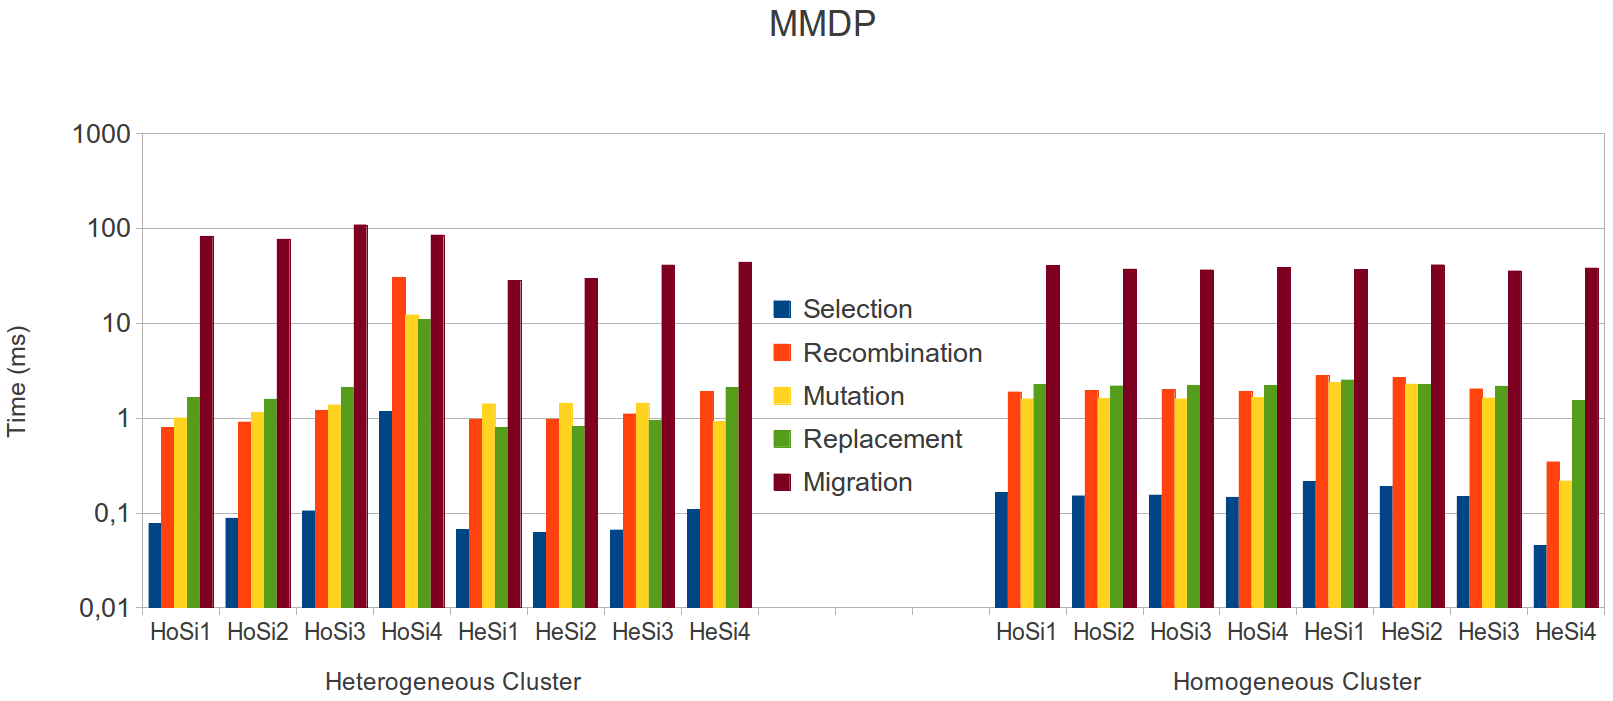
\epsfig{file=images/mmdpbars.eps, width = 14cm}
\caption{Average running time in each stage of the algorithm for the MMDP problem.}
\label{fig:MMDPbars}
\end{figure}

\begin{figure}[htb]
\centering
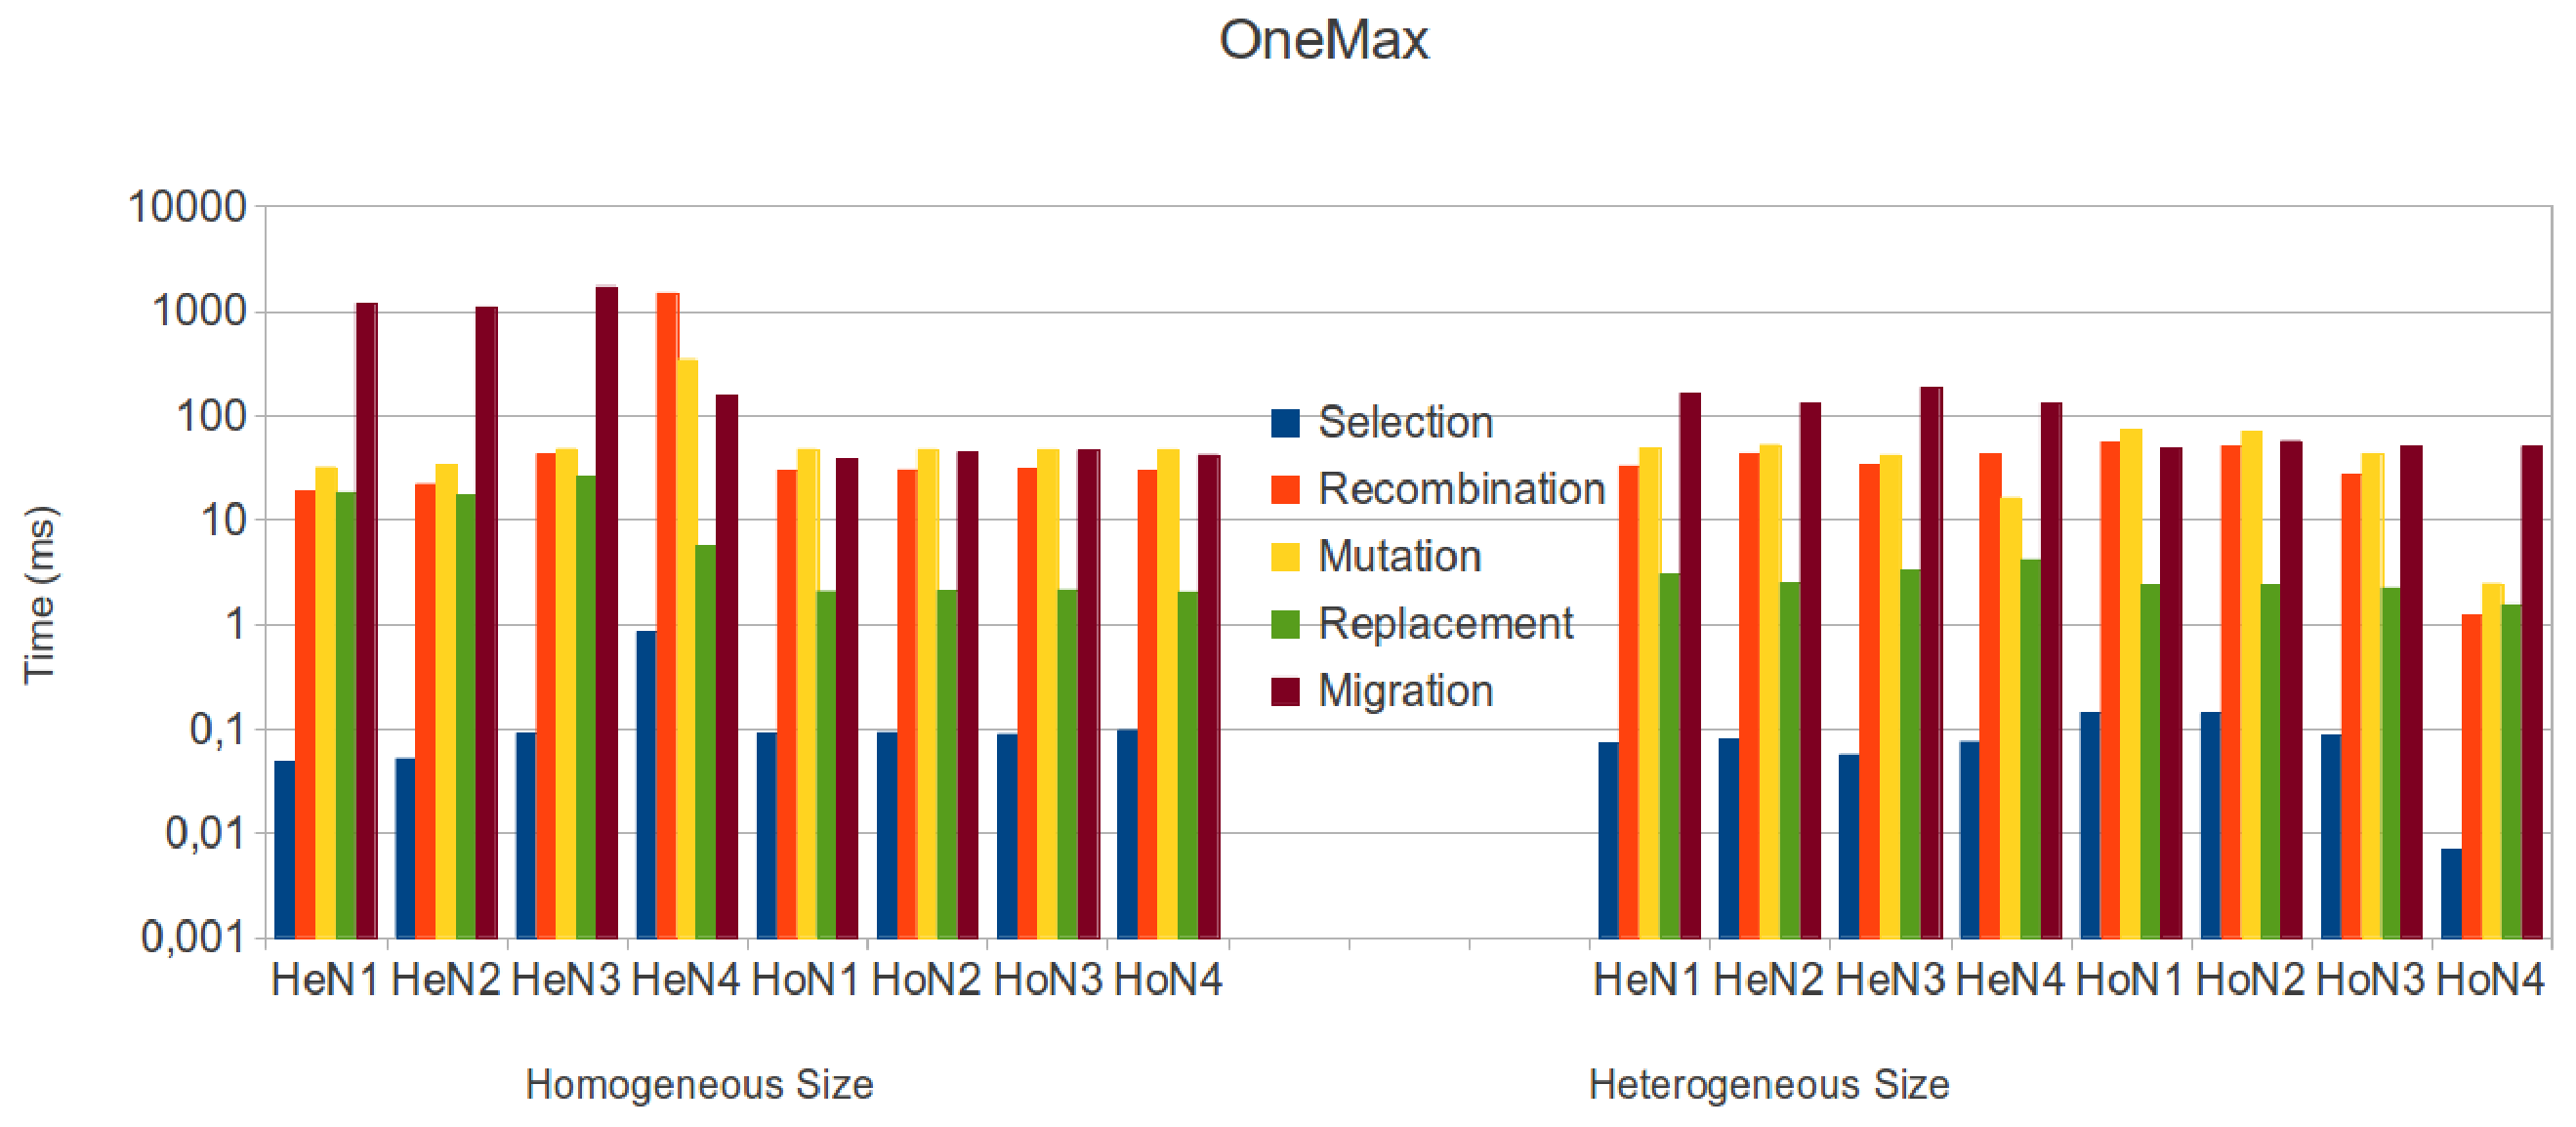
\epsfig{file=images/onemaxbars.eps, width = 14cm}
\caption{Average running time in each stage of the algorithm for the ONEMAX problem.}
\label{fig:ONEMAXbars}
\end{figure}

\begin{table}[htb]
\centering




\caption{Times of the stages of the algorithm for the MMDP problem (in ms).}
\resizebox{14cm}{!}{
\begin{tabular}{|c|c|c|c|c|c|} \hline
\multicolumn{6}{|c|}{Heterogeneous Cluster} \\ \hline
Node	& Selection		& Recombination		& Mutation		& Replacement		& Migration	        \\ \hline
HoSi HeN1    & 0,077 $\pm$  0,170 &  0,788  $\pm$ 0,779  & 1,004  $\pm$ 0,187 &  1,648  $\pm$ 20,185 & 82,458  $\pm$ 143,266 \\ \hline
HoSi HeN2    & 0,088 $\pm$  0,190 &  0,907 $\pm$  0,932  & 1,145  $\pm$ 0,425 &  1,579  $\pm$ 17,907 & 76,725  $\pm$ 126,360\\ \hline
HoSi HeN3    & 0,105 $\pm$  0,163 &  1,207 $\pm$  0,927  & 1,374  $\pm$ 0,301 &  2,108  $\pm$ 21,848 & 108,605 $\pm$ 142,633\\ \hline
HoSi HeN4    & 1,165 $\pm$  1,526 &  30,445$\pm$  59,553 & 12,221 $\pm$ 7,412 &  10,978 $\pm$ 57,135 & 84,936  $\pm$ 0,000\\ \hline \hline
HeSi HeN1    & 0,067 $\pm$  0,065  & 0,973  $\pm$ 0,403 &  1,411 $\pm$  0,166 &  0,790  $\pm$ 6,266 &  28,081 $\pm$ 42,169 \\ \hline
HeSi HeN2    & 0,062 $\pm$  0,075  & 0,973  $\pm$ 0,470 &  1,433 $\pm$  0,265 &  0,811  $\pm$ 7,056 &  29,667 $\pm$ 48,702 \\ \hline
HeSi HeN3    & 0,066 $\pm$  0,108  & 1,104  $\pm$ 0,346 &  1,435 $\pm$  0,296 &  0,937  $\pm$ 7,072 &  40,964 $\pm$ 40,027 \\ \hline
HeSi HeN4    & 0,109 $\pm$  0,257  & 1,895  $\pm$ 5,611 &  0,913 $\pm$  0,834 &  2,085  $\pm$ 5,626 &  43,880 $\pm$ 7,535 \\ \hline 


\multicolumn{6}{|c|}{Homogeneous Cluster} \\ \hline									
Node	& Selection		& Recombination		& Mutation		& Replacement		& Migration	\\ \hline
HoSi HoN1    & 0,163 $\pm$  0,223 &  1,884 $\pm$  2,386  & 1,591  $\pm$ 0,479 &  2,254  $\pm$ 5,513  & 40,256  $\pm$ 8,726\\ \hline
HoSi HoN2    & 0,151 $\pm$  0,212 &  1,952 $\pm$  2,876  & 1,597  $\pm$ 0,574 &  2,178  $\pm$ 4,922  & 37,110  $\pm$ 6,999\\ \hline
HoSi HoN3    & 0,154 $\pm$  0,206 &  1,990 $\pm$  3,010  & 1,591  $\pm$ 0,577 &  2,215  $\pm$ 4,743  & 36,413  $\pm$ 5,266\\ \hline
HoSi HoN4    & 0,146 $\pm$  0,196 &  1,913 $\pm$  2,697  & 1,651  $\pm$ 1,167 &  2,194  $\pm$ 5,124  & 38,429  $\pm$ 6,192\\ \hline \hline
HeSi HoN1    & 0,214 $\pm$  0,288  & 2,800  $\pm$ 3,793 &  2,359 $\pm$  0,691 &  2,516  $\pm$ 4,706 &  36,972 $\pm$ 4,214 \\ \hline
HeSi HoN2    & 0,190 $\pm$  0,252  & 2,672  $\pm$ 3,902 &  2,277 $\pm$  0,649 &  2,261  $\pm$ 4,546 &  41,171 $\pm$ 9,672 \\ \hline
HeSi HoN3    & 0,148 $\pm$  0,208  & 2,030  $\pm$ 3,161 &  1,623 $\pm$  0,500 &  2,164  $\pm$ 4,512 &  35,551 $\pm$  6,132 \\ \hline
HeSi HoN4    & 0,045 $\pm$  0,052  & 0,345  $\pm$ 1,121 &  0,217 $\pm$  0,142 &  1,531  $\pm$ 4,856 &  38,106 $\pm$ 9,251 \\ \hline
\end{tabular}
}
\label{tab:mmdptimes}
\end{table}








\begin{table}[htb]
\centering
\caption{Times of the stages of the algorithm for the OneMax problem (in ms).}
\resizebox{14cm}{!}{
\begin{tabular}{|c|c|c|c|c|c|} \hline
\multicolumn{6}{|c|}{Heterogeneous Cluster} \\ \hline
Node	& Selection		& Recombination		& Mutation		& Replacement		& Migration	        \\ \hline
HoSi HeN1  &  0,048 $\pm$  0,043  & 18,713 $\pm$ 13,454 & 31,984 $\pm$ 2,104  & 18,375 $\pm$ 197,676 & 1172,986  $\pm$  1108,388 \\ \hline
HoSi HeN2  &  0,052 $\pm$  0,051  & 22,266 $\pm$  22,716 & 33,553 $\pm$ 4,931 &  17,176 $\pm$ 180,580 & 1085,508  $\pm$  995,382 \\ \hline
HoSi HeN3  &  0,091 $\pm$  1,005  & 42,634 $\pm$ 21,621  & 47,674 $\pm$ 0,546 &  26,094 $\pm$ 252,667 & 1708,402 $\pm$   1207,925 \\ \hline
HoSi HeN4  &  0,851  $\pm$ 0,435  & 1491,568 $\pm$ 1185,723 & 344,872$\pm$ 6,634 &  5,655  $\pm$ 16,175 & 154,019 $\pm$0,000 \\ \hline \hline
HeSi HeN1 &   0,072 $\pm$  0,063 &  32,917 $\pm$ 26,792 & 49,103 $\pm$ 2,655  & 3,023 $\pm$  27,647 & 163,479 $\pm$157,172 \\ \hline
HeSi HeN2 &   0,080 $\pm$  0,092 &  43,001 $\pm$ 51,680 & 52,288 $\pm$ 13,210 & 2,527 $\pm$  21,861 & 131,063 $\pm$124,404 \\ \hline
HeSi HeN3 &   0,057 $\pm$  0,052 &  33,951 $\pm$ 15,063 & 41,375 $\pm$ 1,707  & 3,284 $\pm$  30,170 & 186,467 $\pm$163,906 \\ \hline
HeSi HeN4 &   0,075 $\pm$  0,107 &  42,443 $\pm$ 88,536 & 16,236 $\pm$ 12,028 & 4,194 $\pm$  33,119 & 131,135 $\pm$144,359 \\ \hline 
\multicolumn{6}{|c|}{Homogeneous Cluster} \\ \hline									
Node	& Selection		& Recombination		& Mutation		& Replacement		& Migration	\\ \hline
HoSi HoN1  &  0,091 $\pm$  0,078  & 29,969 $\pm$ 21,459 & 47,445 $\pm$ 2,194 &  2,073 $\pm$  6,970 &  38,782 $\pm$ 40,369 \\ \hline
HoSi HoN2  &  0,093 $\pm$  0,082  & 30,119 $\pm$ 22,029 & 47,247 $\pm$ 2,146 &  2,108 $\pm$  7,440 &  44,303 $\pm$ 42,759 \\ \hline
HoSi HoN3  &  0,089 $\pm$  0,080  & 30,951 $\pm$ 21,904 & 47,103 $\pm$ 2,031 &  2,138 $\pm$  8,006 &  46,107 $\pm$ 47,351 \\ \hline
HoSi HoN4  &  0,098 $\pm$  0,075  & 29,468 $\pm$ 20,876 & 47,086 $\pm$ 1,856 &  2,043 $\pm$  7,491 &  41,458 $\pm$ 44,970 \\ \hline \hline
HeSi HoN1 &   0,144 $\pm$  0,151 &  56,124 $\pm$ 48,229 & 72,811 $\pm$ 5,177  & 2,424 $\pm$  9,056  & 48,165  $\pm$57,798 \\ \hline
HeSi HoN2 &   0,141 $\pm$  0,152 &  51,226 $\pm$ 41,016 & 70,047 $\pm$ 4,152  & 2,427 $\pm$  10,890 & 57,152  $\pm$74,177 \\ \hline
HeSi HoN3 &   0,086 $\pm$  0,088 &  26,932 $\pm$ 20,460 & 42,963 $\pm$ 3,935  & 2,239 $\pm$  8,658  & 51,014  $\pm$49,648 \\ \hline
HeSi HoN4 &   0,007 $\pm$  0,008 &  1,215  $\pm$ 1,133  & 2,470  $\pm$ 0,098  & 1,553 $\pm$  10,078 & 50,498 $\pm$ 63,983 \\ \hline
\end{tabular}
}
\label{tab:onemaxtimes}
\end{table}

\section{Conclusions}
% no cuentes otra vez lo de los computing trends, hombre. Empieza
% diciendo "in this paper we have introduced this o studied that" - JJ FERGU: Cambiada la introducción
%New computing trends, such as Cloud Computing or Service Oriented
%Architecture are providing a massively amount of heterogeneous
%computational devices. 
%In this paper we have performed a study about adapting the
%population size of a distributed Evolutionary Algorithm to the computational
%power of different nodes in a heterogeneous cluster (a cluster with different hardware).


In this paper we describe a study on the adaptation of the population size of a distributed EA to the computational power of the different nodes of an heterogeneous cluster. The same parameter set has been also tested in a homogeneous cluster. 

Results shows that adapting the population size to the computational power of each node in the heterogeneous cluster yields significantly
better results in time than keeping the same parameter in all nodes. This advantage is due to the combination of the heterogeneous parameters with the heterogeneity of the machines. On the contrary, the same (heterogeneous) parameter set in all islands of the homogeneous cluster could not improve the results than the same parameter in all nodes.

%To obtain a fair parameter configuration,
%this parameter has been obtained proportionally to the attained
%average generations of each node in executions with the same number of
%individuals. Results show that adapting the population size to the computational power decreases
%the execution time significantly in heterogeneous clusters, while
%changing this parameter in homogeneous clusters does not always
%performs better. 

Moreover, changing the population size affects to stages
of the algorithm that are independent of the population size, such as
the migration. 

In this work, we calculate the computational power of each node proportionally 
to the average number of generations for the homogeneous parameter set. These results are a promising start for adapting EAs to the
performance of each execution node, using more adequate benchmarks or in a dynamic way. 
% Falta una discusión sobre si las mejoras se deben exclusivamente al
% número de evaluaciones o hay algún otro factor ¿menos overhead?
% ¿nodos más rápidos? - JJ FERGU: no, de hecho el número de evaluaciones no siempre disminuye, lo digo arriba.

In the future it would be interesting to check the scalability of this
approach, using more computational nodes and larger problem
instances. In addition, other parameters such as migration rate or
crossover probability could be adapted to the execution
nodes. Different benchmarks will be also used to lead to automatic
parameter adaptation in runtime (online), with different nodes entering or
exiting in the topology, or adapting the parameters to the current load of the
system. 

\section*{Acknowledgements}
This work has been supported in part by FPU research grant AP2009-2942 and projects EvOrq (TIC-3903), CANUBE (CEI2013-P-14) and ANYSELF (TIN2011-28627-C04-02).
%% The Appendices part is started with the command \appendix;
%% appendix sections are then done as normal sections
%% \appendix

%% \section{}
%% \label{}

%% References
%%
%% Following citation commands can be used in the body text:
%% Usage of \cite is as follows:
%%   \cite{key}         ==>>  [#]
%%   \cite[chap. 2]{key} ==>> [#, chap. 2]
%%

%% References with bibTeX database:

%\bibliographystyle{elsarticle-num}
%\bibliography{AMIVITAL-ESA}

%% Authors are advised to submit their bibtex database files. They are
%% requested to list a bibtex style file in the manuscript if they do
%% not want to use elsarticle-num.bst.

%% References without bibTeX database:

% \begin{thebibliography}{00}

%% \bibitem must have the following form:
%%   \bibitem{key}...
%%

% \bibitem{}

% \end{thebibliography}

\bibliographystyle{plain}
\bibliography{heterogeneous}

\end{document}

%%
%% End of file `elsarticle-template-num.tex'.
